\begin{figure}[!htbp]
  \centering
  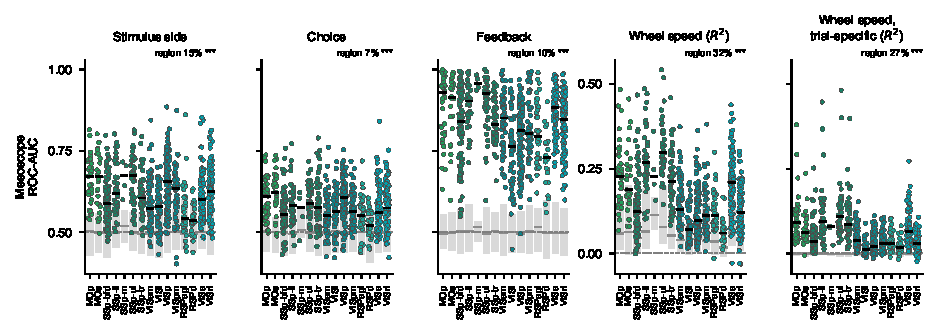
\includegraphics[width=\linewidth,height=0.8\textheight,keepaspectratio]{figures/meso_fixed_200_regions.pdf}
  \caption{All-neuron and fixed-size mesoscope decoding by Beryl region. Black bars are region medians. Dashed lines mark chance, and grey bands and lines show the 5th--95th percentiles and medians of the trial-shuffle nulls. Both rows use the same score axes. Insets give the region share from the crossed region, session and animal model. Stars indicate likelihood-ratio $p<0.05$, $p<0.01$ and $p<0.001$. \textbf{a} All-neuron mesoscope row from \figref{region_variance}a, including its original trial-shuffle baselines and mixed-model estimates with log neuron count. It uses 149 sessions and 989--996 session--region pairs per target. \textbf{b} Decoding from 200 randomly sampled neurons per pair, using one seeded draw from each of 821 matched pairs across 148 sessions. The null uses one joint trial-label shuffle per session with the same sampled neurons. The mixed model has a fixed neuron count.}
  \label{fig:meso_fixed_200_regions}
\end{figure}
